% -*- coding: utf-8 -*-
% !TEX program = xelatex

\documentclass[11pt]{beamer}

%\usetheme[style=beta]{epyt} % alpha, beta, delta, gamma, zeta
% \usetheme{Warsaw}
\usetheme{PaloAlto}
% \usecolortheme{albatross}

\usepackage[UTF8,noindent]{ctex}
% ######### DEFINE COLOR ###############
\definecolor{red}{HTML}{E55C5C}
\definecolor{cyan}{HTML}{5CE6E5}
 
\def\cyan{\textcolor{cyan}}
\def\red{\textcolor{red}}

\def\ds{\displaystyle}
\def\cd{\cdots}
\def\dd{\ddots}
\def\vd{\vdots}
\def\id{\iddots}
\def\ft{\frametitle}
\def\diag{\mathrm{diag}}
\def\Im{\mathrm{Im~}}
\def\Ker{\mathrm{Ker~}}

\def\MA{\boldsymbol{A}}
\def\MB{\boldsymbol{B}}
\def\MC{\boldsymbol{C}}
\def\MD{\boldsymbol{D}}
\def\ME{\boldsymbol{E}}
\def\MF{\boldsymbol{F}}
\def\MG{\boldsymbol{G}}
\def\MH{\boldsymbol{H}}
\def\MI{\boldsymbol{I}}
\def\MP{\boldsymbol{P}}
\def\MQ{\boldsymbol{Q}}
\def\MR{\boldsymbol{R}}
\def\MS{\boldsymbol{S}}
\def\MT{\boldsymbol{T}}
\def\MU{\boldsymbol{U}}
\def\MX{\boldsymbol{X}}
\def\MY{\boldsymbol{Y}}
\def\MZ{\boldsymbol{Z}}
\def\M0{\boldsymbol{0}}
\def\MLambda{\boldsymbol{\Lambda}}

\def\R{\mathbb R}
\def\C{\mathbb C}
\def\dim{\mathrm{dim~}}
\def\rank{\mathrm{r}}
\def\tr{\mathrm{tr}}
\def\det{\mathrm{det}}
\def\vn{{\boldsymbol{n}}}
\def\vx{{\boldsymbol{x}}}
\def\vy{{\boldsymbol{y}}}
\def\vz{{\boldsymbol{z}}}
\def\va{{\boldsymbol{a}}}
\def\vb{{\boldsymbol{b}}}
\def\ve{{\boldsymbol{e}}}
\def\vi{{\boldsymbol{i}}}
\def\vj{{\boldsymbol{j}}}
\def\vk{{\boldsymbol{k}}}
\def\vu{{\boldsymbol{u}}}
\def\vv{{\boldsymbol{v}}}

\def\tf{\ttfamily}
\def\Lambdabd{\boldsymbol{\Lambda}}
\def\alphabd{\boldsymbol{\alpha}}
\def\betabd{\boldsymbol{\beta}}
\def\gammabd{\boldsymbol{\gamma}}
\def\xibd{\boldsymbol{\xi}}
\def\zetabd{\boldsymbol{\zeta}}
\def\etabd{\boldsymbol{\eta}}
\def\epsilonbd{\boldsymbol{\epsilon}}
\def\phibd{\boldsymbol{\phi}}
\def\varphibd{\boldsymbol{\varphi}}
\def\sigmabd{\boldsymbol{\sigma}}
\def\omegabd{\boldsymbol{\omega}}
\def\taubd{\boldsymbol{\tau}}
%\def\rank{\boldsymbol{rank}}
\usepackage{amsmath,amsthm,amssymb,mathdots}
\usepackage{fourier}
\usepackage{multicol}
%\usepackage{fontspec}
\usepackage{subfigure}
\usepackage[most]{tcolorbox}
\newcounter{testexample}
\usepackage{xparse}
\usepackage{lipsum}
\usepackage[UTF8,noindent]{ctex}
\usepackage{extarrows}
%\usepackage{courier}
\usepackage{animate}
\usepackage{dcolumn}
\usepackage{pgf}
\usepackage{tikz}
\usetikzlibrary{calc}
\usetikzlibrary{arrows,snakes,backgrounds,shapes,patterns}
\usetikzlibrary{matrix,fit,positioning,decorations.pathmorphing}
\usepackage{listings}
\lstset{
        language=c,
        keywordstyle=\color{red},
        frame=tb,
        basicstyle=\ttfamily,
        commentstyle=\small\color{blue},
        breakindent=0pt,
        rulesepcolor=\color{red!20!green!20!blue!20},
        rulecolor=\color{black},
        tabsize=4,
        numbersep=5pt,
        breaklines=true,
        backgroundcolor=\color{red!10},
        showstringspaces=false,
        showspaces=false,
        showtabs=false,
        extendedchars=false,
        escapeinside=``,
}

\usepackage{refcount}
\usepackage{multicol}
\newcounter{countitems}
\newcounter{nextitemizecount}
\newcommand{\setupcountitems}{%
	\stepcounter{nextitemizecount}%
	\setcounter{countitems}{0}%
	\preto\item{\stepcounter{countitems}}%
}
\makeatletter
\newcommand{\computecountitems}{%
	\edef\@currentlabel{\number\c@countitems}%
	\label{countitems@\number\numexpr\value{nextitemizecount}-1\relax}%
}
\newcommand{\nextitemizecount}{%
	\getrefnumber{countitems@\number\c@nextitemizecount}%
}
\newcommand{\previtemizecount}{%
	\getrefnumber{countitems@\number\numexpr\value{nextitemizecount}-1\relax}%
}
\makeatother    
\newenvironment{AutoMultiColItemize}{%
	\ifnumcomp{\nextitemizecount}{>}{3}{\begin{multicols}{2}}{}%
		\setupcountitems\begin{itemize}}%
		{\end{itemize}%
		\unskip\computecountitems\ifnumcomp{\previtemizecount}{>}{3}{\end{multicols}}{}}

\def\exampletext{例} % If English
\NewDocumentEnvironment{testexample}{ O{} }
{
\colorlet{colexam}{red!55!black} % Global example color
\newtcolorbox[use counter=testexample]{testexamplebox}{%
    % Example Frame Start
    empty,% Empty previously set parameters
    title={\exampletext: #1},% use \thetcbcounter to access the testexample counter text
    % Attaching a box requires an overlay
    attach boxed title to top left,
       % Ensures proper line breaking in longer titles
       minipage boxed title,
    % (boxed title style requires an overlay)
    boxed title style={empty,size=minimal,toprule=0pt,top=4pt,left=3mm,overlay={}},
    coltitle=colexam,fonttitle=\bfseries,
    before=\par\medskip\noindent,parbox=false,boxsep=0pt,left=3mm,right=0mm,top=2pt,breakable,pad at break=0mm,
       before upper=\csname @totalleftmargin\endcsname0pt, % Use instead of parbox=true. This ensures parskip is inherited by box.
    % Handles box when it exists on one page only
    overlay unbroken={\draw[colexam,line width=.5pt] ([xshift=-0pt]title.north west) -- ([xshift=-0pt]frame.south west); },
    % Handles multipage box: first page
    overlay first={\draw[colexam,line width=.5pt] ([xshift=-0pt]title.north west) -- ([xshift=-0pt]frame.south west); },
    % Handles multipage box: middle page
    overlay middle={\draw[colexam,line width=.5pt] ([xshift=-0pt]frame.north west) -- ([xshift=-0pt]frame.south west); },
    % Handles multipage box: last page
    overlay last={\draw[colexam,line width=.5pt] ([xshift=-0pt]frame.north west) -- ([xshift=-0pt]frame.south west); },%
    }
\begin{testexamplebox}}
{\end{testexamplebox}\endlist}
\renewcommand{\proofname}{\textbf{证明}}
\newtheorem{li}{例}%[section]
%\newtheorem*{li*}{例}
\newtheorem{lianxi}{练习}
\newtheorem*{jielun}{结论}
\newtheorem*{dingli}{定理}
\newtheorem*{mingti}{{命题}} 
\newtheorem*{yinli}{{引理}} 
\newtheorem*{tuilun}{{推论}}
\newtheorem*{dingyi}{{定义}}
\newtheorem*{biancheng}{{编程}}
\newtheorem*{jie}{{解}}
\newtheorem{zhu}{{注}}
\newtheorem*{xingzhi}{{性质}}%[subsection]
\newtheorem*{wenti}{{问题}}
\newtheorem*{rem}{{Remark}}
\newtheorem*{lem}{{Lemma}}



\begin{document}
\title{C语言}
\subtitle{数组与指针}

\author{张晓平}
\institute{武汉大学数学与统计学院
}


\begin{frame}[plain]\transboxout
  \titlepage
\end{frame}

%\section*{目录}
%\begin{frame}\ft{\secname}
%    \tableofcontents
%\end{frame}


\section{数组回顾}

\begin{frame}[fragile]\ft{数组}
数组由一系列类型相同的元素组成,数组声明必须包括元素的个数(即数组长度)与类型。如

\begin{lstlisting}
float farray[20];
char carray[12];
int iarray[50];
\end{lstlisting}
\end{frame}

\begin{frame}[fragile]\ft{数组初始化}
\begin{figure}
\centering
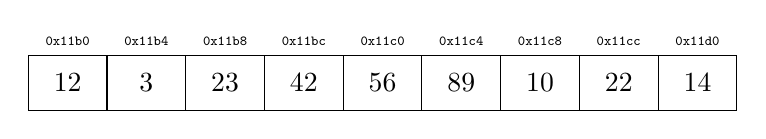
\begin{tikzpicture}
\draw (0,0) rectangle node[] {12} (1,0.7); \node at (0.5,0.7) [above] {\tf \tiny 0x11b0};
\draw (1,0) rectangle node[] {3} (2,0.7);  \node at (1.5,0.7) [above] {\tf \tiny 0x11b4};
\draw (2,0) rectangle node[] {23} (3,0.7); \node at (2.5,0.7) [above] {\tf \tiny 0x11b8};
\draw (3,0) rectangle node[] {42} (4,0.7); \node at (3.5,0.7) [above] {\tf \tiny 0x11bc};
\draw (4,0) rectangle node[] {56} (5,0.7); \node at (4.5,0.7) [above] {\tf \tiny 0x11c0};
\draw (5,0) rectangle node[] {89} (6,0.7); \node at (5.5,0.7) [above] {\tf \tiny 0x11c4};
\draw (6,0) rectangle node[] {10} (7,0.7); \node at (6.5,0.7) [above] {\tf \tiny 0x11c8};
\draw (7,0) rectangle node[] {22} (8,0.7); \node at (7.5,0.7) [above] {\tf \tiny 0x11cc};
\draw (8,0) rectangle node[] {14} (9,0.7); \node at (8.5,0.7) [above] {\tf \tiny 0x11d0};
\end{tikzpicture}
\end{figure}

$$
\Big\downarrow  \mbox{\lstinline|int array[5];|}
$$


\begin{figure}
\centering
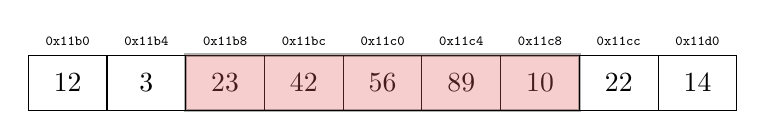
\begin{tikzpicture}
\draw (0,0) rectangle node[] {12} (1,0.7); \node at (0.5,0.7) [above] {\tf \tiny 0x11b0};
\draw (1,0) rectangle node[] {3} (2,0.7);  \node at (1.5,0.7) [above] {\tf \tiny 0x11b4};
\draw (2,0) rectangle node[] {23} (3,0.7); \node at (2.5,0.7) [above] {\tf \tiny 0x11b8};
\draw (3,0) rectangle node[] {42} (4,0.7); \node at (3.5,0.7) [above] {\tf \tiny 0x11bc};
\draw (4,0) rectangle node[] {56} (5,0.7); \node at (4.5,0.7) [above] {\tf \tiny 0x11c0};
\draw (5,0) rectangle node[] {89} (6,0.7); \node at (5.5,0.7) [above] {\tf \tiny 0x11c4};
\draw (6,0) rectangle node[] {10} (7,0.7); \node at (6.5,0.7) [above] {\tf \tiny 0x11c8};
\draw (7,0) rectangle node[] {22} (8,0.7); \node at (7.5,0.7) [above] {\tf \tiny 0x11cc};
\draw (8,0) rectangle node[] {14} (9,0.7); \node at (8.5,0.7) [above] {\tf \tiny 0x11d0};

\draw[opacity=0.3, fill=red, very thick] (2,0) rectangle (7,0.7);
\end{tikzpicture}
\end{figure}


\pause 

{\bf 数组名表示的是数组首元素的地址。故\lstinline| array |的值为\lstinline| 0x11b8 |。}

\end{frame}


\begin{frame}[fragile]\ft{数组初始化}
\begin{figure}
\centering
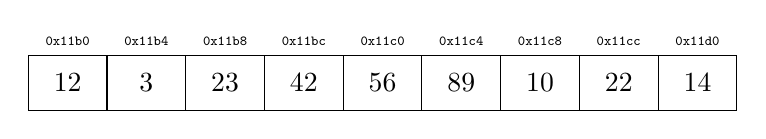
\begin{tikzpicture}
\draw (0,0) rectangle node[] {12} (1,0.7); \node at (0.5,0.7) [above] {\tf \tiny 0x11b0};
\draw (1,0) rectangle node[] {3} (2,0.7);  \node at (1.5,0.7) [above] {\tf \tiny 0x11b4};
\draw (2,0) rectangle node[] {23} (3,0.7); \node at (2.5,0.7) [above] {\tf \tiny 0x11b8};
\draw (3,0) rectangle node[] {42} (4,0.7); \node at (3.5,0.7) [above] {\tf \tiny 0x11bc};
\draw (4,0) rectangle node[] {56} (5,0.7); \node at (4.5,0.7) [above] {\tf \tiny 0x11c0};
\draw (5,0) rectangle node[] {89} (6,0.7); \node at (5.5,0.7) [above] {\tf \tiny 0x11c4};
\draw (6,0) rectangle node[] {10} (7,0.7); \node at (6.5,0.7) [above] {\tf \tiny 0x11c8};
\draw (7,0) rectangle node[] {22} (8,0.7); \node at (7.5,0.7) [above] {\tf \tiny 0x11cc};
\draw (8,0) rectangle node[] {14} (9,0.7); \node at (8.5,0.7) [above] {\tf \tiny 0x11d0};
\end{tikzpicture}
\end{figure}

$$
\Big\downarrow  \mbox{\lstinline|int array[5] = {1,2,3};|}
$$


\begin{figure}
\centering
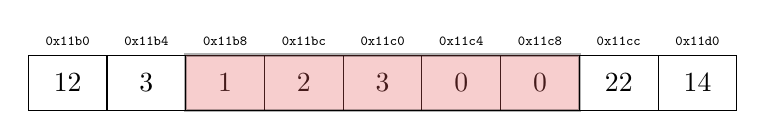
\begin{tikzpicture}
\draw (0,0) rectangle node[] {12} (1,0.7); \node at (0.5,0.7) [above] {\tf \tiny 0x11b0};
\draw (1,0) rectangle node[] {3} (2,0.7);  \node at (1.5,0.7) [above] {\tf \tiny 0x11b4};
\draw (2,0) rectangle node[] {1} (3,0.7); \node at (2.5,0.7) [above] {\tf \tiny 0x11b8};
\draw (3,0) rectangle node[] {2} (4,0.7); \node at (3.5,0.7) [above] {\tf \tiny 0x11bc};
\draw (4,0) rectangle node[] {3} (5,0.7); \node at (4.5,0.7) [above] {\tf \tiny 0x11c0};
\draw (5,0) rectangle node[] {0} (6,0.7); \node at (5.5,0.7) [above] {\tf \tiny 0x11c4};
\draw (6,0) rectangle node[] {0} (7,0.7); \node at (6.5,0.7) [above] {\tf \tiny 0x11c8};
\draw (7,0) rectangle node[] {22} (8,0.7); \node at (7.5,0.7) [above] {\tf \tiny 0x11cc};
\draw (8,0) rectangle node[] {14} (9,0.7); \node at (8.5,0.7) [above] {\tf \tiny 0x11d0};
\draw[opacity=0.3, fill=red, very thick] (2,0) rectangle (7,0.7);
\end{tikzpicture}
\end{figure}

\end{frame}


\begin{frame}[fragile]\ft{数组初始化}
\begin{figure}
\centering
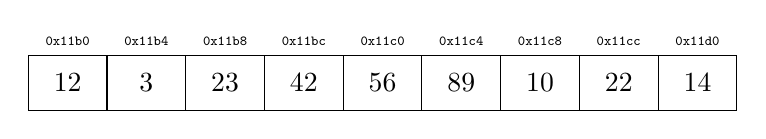
\begin{tikzpicture}
\draw (0,0) rectangle node[] {12} (1,0.7); \node at (0.5,0.7) [above] {\tf \tiny 0x11b0};
\draw (1,0) rectangle node[] {3} (2,0.7);  \node at (1.5,0.7) [above] {\tf \tiny 0x11b4};
\draw (2,0) rectangle node[] {23} (3,0.7); \node at (2.5,0.7) [above] {\tf \tiny 0x11b8};
\draw (3,0) rectangle node[] {42} (4,0.7); \node at (3.5,0.7) [above] {\tf \tiny 0x11bc};
\draw (4,0) rectangle node[] {56} (5,0.7); \node at (4.5,0.7) [above] {\tf \tiny 0x11c0};
\draw (5,0) rectangle node[] {89} (6,0.7); \node at (5.5,0.7) [above] {\tf \tiny 0x11c4};
\draw (6,0) rectangle node[] {10} (7,0.7); \node at (6.5,0.7) [above] {\tf \tiny 0x11c8};
\draw (7,0) rectangle node[] {22} (8,0.7); \node at (7.5,0.7) [above] {\tf \tiny 0x11cc};
\draw (8,0) rectangle node[] {14} (9,0.7); \node at (8.5,0.7) [above] {\tf \tiny 0x11d0};
\end{tikzpicture}
\end{figure}

$$
\Big\downarrow  \mbox{\lstinline|int array[5] = {2, [2]=5, 6, [0]=8};|}
$$


\begin{figure}
\centering
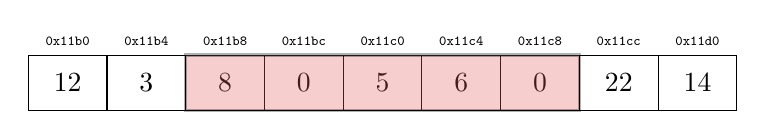
\begin{tikzpicture}
\draw (0,0) rectangle node[] {12} (1,0.7); \node at (0.5,0.7) [above] {\tf \tiny 0x11b0};
\draw (1,0) rectangle node[] {3} (2,0.7);  \node at (1.5,0.7) [above] {\tf \tiny 0x11b4};
\draw (2,0) rectangle node[] {8} (3,0.7); \node at (2.5,0.7) [above] {\tf \tiny 0x11b8};
\draw (3,0) rectangle node[] {0} (4,0.7); \node at (3.5,0.7) [above] {\tf \tiny 0x11bc};
\draw (4,0) rectangle node[] {5} (5,0.7); \node at (4.5,0.7) [above] {\tf \tiny 0x11c0};
\draw (5,0) rectangle node[] {6} (6,0.7); \node at (5.5,0.7) [above] {\tf \tiny 0x11c4};
\draw (6,0) rectangle node[] {0} (7,0.7); \node at (6.5,0.7) [above] {\tf \tiny 0x11c8};
\draw (7,0) rectangle node[] {22} (8,0.7); \node at (7.5,0.7) [above] {\tf \tiny 0x11cc};
\draw (8,0) rectangle node[] {14} (9,0.7); \node at (8.5,0.7) [above] {\tf \tiny 0x11d0};

\draw[opacity=0.3, fill=red, very thick] (2,0) rectangle (7,0.7);
\end{tikzpicture}
\end{figure}

\end{frame}


\section{指针}
\begin{frame}[fragile]\ft{\secname}
\begin{itemize}
\item
计算机的硬件指令很大程度上依赖于地址,而指针为我们使用地址提供了一种方法。\\[0.1in]
\item
使用指针能让我们以类似于计算机底层的方式来表达意愿,从而让程序能更高效地工作。\\[0.1in]
\item 
需要强调的是,指针能非常有效地处理数组。事实上,\red{数组是一种变相使用指针的形式。}
\end{itemize}
\end{frame}


\begin{frame}[fragile]\ft{\secname}
再一次强调:\red{数组名是数组首元素的地址。}
\pause \vspace{0.2in}

若\lstinline| array |为一个数组,则以下关系式为真:
\begin{lstlisting}[language=c,backgroundcolor=\color{red!20}]
array == &array[0];
\end{lstlisting}
\end{frame}


\begin{frame}[fragile,allowframebreaks]\ft{\secname}
  \lstinputlisting
  [language=c,numbers=left,frame=single]
  {ch10/code/pnt_add.c}
\end{frame}


\begin{frame}[fragile]\ft{\secname}

\begin{lstlisting}[backgroundcolor=\color{red!20}]
               short double
pointers + 0: 0xf7d0 0xf7b0
pointers + 1: 0xf7d2 0xf7b8
pointers + 2: 0xf7d4 0xf7c0
pointers + 3: 0xf7d6 0xf7c8
\end{lstlisting}
\end{frame}


\begin{frame}[fragile]\ft{\secname}
在C中,对指针加1的结果是对该指针增加一个存储单元。对数组而言,地址会增加到下一个元素的地址,而不是下一个字节。
\end{frame}


\begin{frame}[fragile]\ft{\secname}
\begin{center}
\red{\Large 指针定义小结}
\end{center}
\begin{itemize}
\item 
指针的数值就是它所指向的对象的地址。地址的内部表达方式由硬件决定,很多计算机都是以字节编址的。 \\[0.1in]
\item
在指针前用运算符\lstinline| * |就可以得到该指针所指向的对象的值。\\[0.1in]
\item
对指针加1,等价于对指针的值加上它所指向的对象的字节大小。
\end{itemize}
\end{frame}


\begin{frame}[fragile]\ft{\secname}
\begin{lstlisting}[language=c,backgroundcolor=\color{red!20}]
dates + 2 == &dates[2];    // same address
*(dates + 2) == dates[2];  // same value
\end{lstlisting}

可以用指针标识数组的每个元素,并得到每个元素的值。从本质上讲,这是对同一对象采用了两种不同的符号表示方法。

\end{frame}


\begin{frame}[fragile]\ft{\secname}
在描述数组时,C确实借助了指针的概念。例如,定义\lstinline| array[n] |时,\vspace{0.1in}

\begin{itemize}
\item
即:\lstinline| *(array + n) |, \\[0.1in]
\item
含义:“寻址到内存中的\lstinline| array |,然后移动\lstinline| n |个单元,再取出数值”。
\end{itemize}
\end{frame}


\begin{frame}[fragile]\ft{\secname}
请注意\lstinline| *(dates+2) |和\lstinline| *dates+2 |的区别。\red{取值运算符\lstinline| * |的优先级高于\lstinline| + |},故后者等价于\lstinline| (*dates)+2 |。\vspace{0.1in}

\begin{lstlisting}[language=c,backgroundcolor=\color{red!20}]
*(dates + 2)  //  same as dates[2]
*dates + 2    //  same as dates[0] + 2
\end{lstlisting}
\end{frame}
 

\section{数组、指针与函数}

\begin{frame}[fragile]\ft{\secname}
编写函数,求一个数组的各元素之和。
\end{frame}

\begin{frame}[fragile]\ft{\secname}
方式一:在函数中给定固定的数组大小。
\begin{lstlisting}[language=c,backgroundcolor=\color{red!20}]
int sum(int * ar)
{
  int i, total = 0;
  
  for (i = 0; i < 10; i++)
    total += ar[i];  
  return total;  
}
\end{lstlisting} \pause 
但该函数仅在数组长度为10时可工作。
\end{frame}

\begin{frame}[fragile]\ft{\secname}
方式二:将数组大小作为参数传递给函数。
\begin{lstlisting}[language=c,backgroundcolor=\color{red!20}]
int sum(int * ar, int n)
{
  int i, total = 0;
  
  for (i = 0; i < n; i++)
    total += ar[i];  
  return total;  
}
\end{lstlisting} \pause 
该方式更为灵活,第一个参数把数组地址和数组类型的信息传递给函数,第二个参数把数组的元素个数传递给函数。
\end{frame}

\begin{frame}[fragile]\ft{\secname}
给定数组
\begin{lstlisting}[language=c,backgroundcolor=\color{red!20},frame=no]
int ar[5] = {1, 2, 3, 4, 5};
\end{lstlisting}
\begin{itemize}
\item 可以求数组的整体和,如
\begin{lstlisting}[language=c,backgroundcolor=\color{red!20},frame=no]
int result = sum(ar, 5);
\end{lstlisting}
\item 也可以求数组的部分和,如
\begin{lstlisting}[language=c,backgroundcolor=\color{red!20},frame=no]
int result = sum(ar+1, 3);
\end{lstlisting}
计算的是\lstinline|ar|的第2个至第4个元素之和。
\end{itemize}

\end{frame}




\begin{frame}[fragile]\ft{\secname}
在做函数声明时,以下四种函数原型是等价的:
\begin{lstlisting}[language=c,backgroundcolor=\color{red!20}]
int sum(int * ar, int n);
int sum(int *, int);

int sum(int ar[], int n);
int sum(int [], int);
\end{lstlisting}
\end{frame}

\begin{frame}[fragile]\ft{\secname}
在定义函数时,名称不可以省略。故在定义时以下两种形式是等价的:
\begin{lstlisting}[language=c,backgroundcolor=\color{red!20}]
int sum(int * ar, int n)
{
  ...
}

int sum(int ar[], int n)
{
  ...
}
\end{lstlisting}
\end{frame}


\end{document}
